\documentclass[t, notes, xcolor=table]{beamer}

\usepackage{wrapfig}
\usepackage{float}
% For tabs in verbatim
\usepackage{fancyvrb}

% Adjust position of the image
\usepackage[export]{adjustbox}

% set fonts
\usefonttheme{professionalfonts} % using non standard fonts for beamer
\usepackage{txfonts,mathptmx}

% set indend spacing for first and second level indentation
\setlength{\leftmargini}{0.5cm}
\setlength{\leftmarginii}{0.5cm}
\setlength{\leftmarginiii}{0.5cm}

% Set circles for bullets 
\setbeamertemplate{itemize items}[circle]

% colors
\usepackage{xcolor}

% multiple columns
\usepackage{multicol}

% todo lists
\usepackage{pifont}
\usepackage{amssymb}

% increase space between text and frame name
\addtobeamertemplate{frametitle}{}{\vspace{0.5em}}

%Information to be included in the title page:
\title{Using Verilog Operators}
\author{Nikola Petrovic}
\institute{University of Belgrade, School of Electrical Engineering}
\date{2022}



\begin{document}

\frame{\titlepage}

%%%%%%%%%%%%%%%%%%%%%%%%%%%%%%%%%%%%%%%%%%%%%%%%%%%%%%%%%%%%
\begin{frame}
\frametitle{Module Objective}

In this module we will choose and use the Verilog operators correctly.

\begin{figure}[H!]
    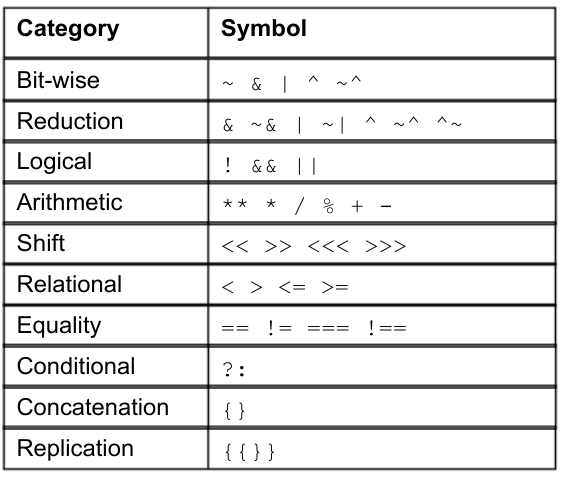
\includegraphics[width=0.5\textwidth]{img/05_operators.png}
\end{figure}

\end{frame}

%%%%%%%%%%%%%%%%%%%%%%%%%%%%%%%%%%%%%%%%%%%%%%%%%%%%%%%%%%%%
\begin{frame}[fragile]
\frametitle{Bit-Wise Operators}
\scriptsize{
\begin{multicols}{2}
\begin{itemize}
\item Bit-wise operators operate on vectors
\item Operations are performed bit by bit on individual bits
\item Unknown bits in an operand do not necessarily lead to unknown bits in result
\end{itemize}
\vfill
\begin{Verbatim}[commandchars=\\\{\}, tabsize=2]
\textcolor{purple}{not  ~}
\textcolor{purple}{and  &}
\textcolor{purple}{or   |}
\textcolor{purple}{xor  ^}
\textcolor{purple}{xnor ~^}
\textcolor{purple}{xnor ^~}
\end{Verbatim}

\columnbreak
\begin{figure}
    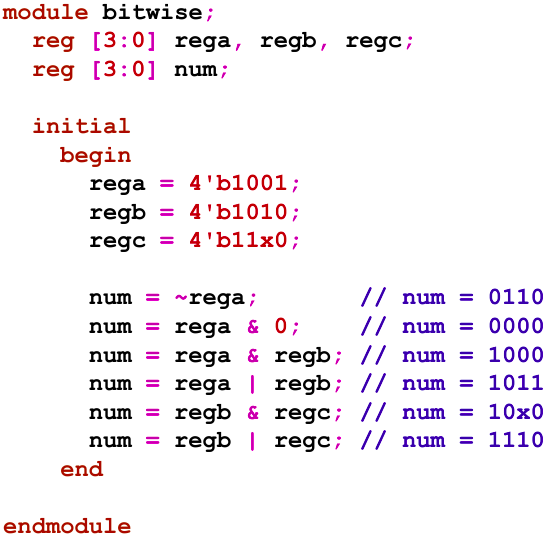
\includegraphics[width=0.45\textwidth]{img/05_bitwise.png}
\end{figure}
\end{multicols}
}
\end{frame}

\note{
\scriptsize{
The bitwise operators perform logical operations in a bitwise manner.
\newline

The bitwise unary negation operator inverts the logical sense of each bit of its operand. Each 0 becomes 1 and each 1 becomes 0, and each high-impedance bit becomes unknown.
\newline

The bitwise binary operators first zero-extend a smaller operand to match the width of a larger operand, and them perform logical operations on individual bit positions. Depending upon the operation, bits in one operand that are 0 or 1 can mask bits in the same position of the other operand that are high-impedance or unknown, so unknown bits in an operand do not necessarily produce unknown bits in the result.

}
}
%%%%%%%%%%%%%%%%%%%%%%%%%%%%%%%%%%%%%%%%%%%%%%%%%%%%%%%%%%%%
\begin{frame}[fragile]
\frametitle{Unary Reduction Operators}
\scriptsize{
\begin{multicols}{2}
\begin{itemize}
\item Reduction operators perform a bit-wise operation on all the bits of a single operand.
\item The result is always \verb+1'b0+, \verb+1'b1+ or \verb+1'bX+  
\end{itemize}
\vfill
\begin{Verbatim}[commandchars=\\\{\}, tabsize=2]
\textcolor{purple}{and  &}
\textcolor{purple}{or   |}
\textcolor{purple}{xor  ^}
\textcolor{purple}{nand ~&}
\textcolor{purple}{nor  ~|}
\textcolor{purple}{xnor ~^}
\textcolor{purple}{xnor ^~}
\end{Verbatim}

\columnbreak
\begin{figure}
    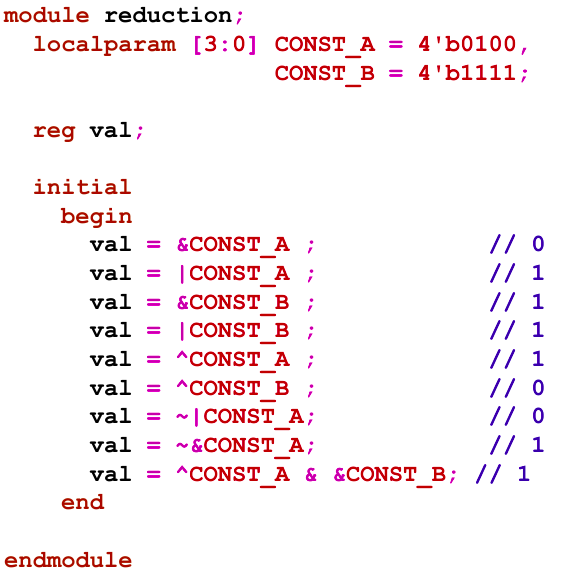
\includegraphics[width=0.45\textwidth]{img/05_reduction.png}
\end{figure}
\end{multicols}
}
\end{frame}
\note{
\footnotesize{
Unary reduction operators operate on all bits of a single operand to produce a single-bit result. The effect is as if the first applied the logical operation to the first two bits of the operand, then iteratively applied the logical operation to the current partial result and the next bit. The result of the operation is always a single bit that is 0, 1 or unknown (x).
\newline

We will see these same operators also used as bitwise binary operators. When used with single operand, they are reduction operators.

}
}

%%%%%%%%%%%%%%%%%%%%%%%%%%%%%%%%%%%%%%%%%%%%%%%%%%%%%%%%%%%%
\begin{frame}[fragile]
\frametitle{Logical Operators}
\scriptsize{
\begin{multicols}{2}
Logical operators interpret their operands as either true (1'b1), false (1'b0) or unknown (1'bX):
\begin{itemize}
\item 0: If all bits 0
\item 1: If any bit 1
\item X: If any bit is X or Z and no bits are 1
\end{itemize}
\vspace{6pt}
\begin{Verbatim}[commandchars=\\\{\}, tabsize=2]
\textcolor{purple}{not !}
\textcolor{purple}{and &&}
\textcolor{purple}{or  ||}
\end{Verbatim}
\vfill
\columnbreak
\begin{figure}
    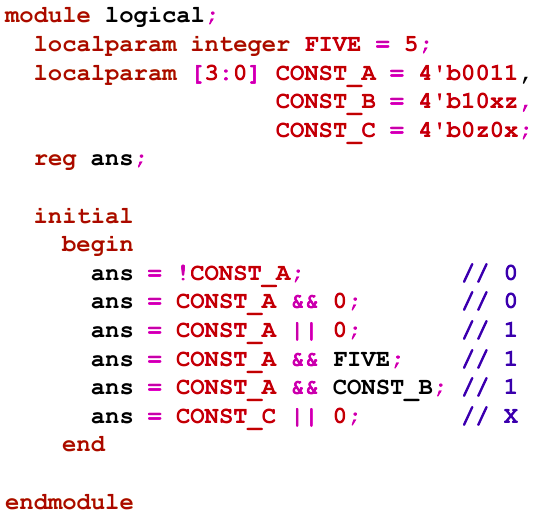
\includegraphics[width=0.45\textwidth]{img/05_logical.png}
\end{figure}
\end{multicols}
}
\end{frame}
\note{
\scriptsize{
Logical operators reduce each operand to a single bit, and then perform a single bit operation.
\newline

The rules for reduction of an operand are as follows:
\begin{itemize}
\item If the operand contains all zeroes, it reduces to logic 0.
\item If the operand contains any ones, it reduces to logic 1.
\item If the operand contain no ones, but does contain one or more high-impedance or unknown values, it reduces to unknown, because its logical values is unknown.
\end{itemize}

The unary logical negation operator then inverts the logical sense of its operand. 0 becomes 1, and 1 becomes 0.
\newline

The binary conjunction  and disjunction operators produce the logical conjunction and disjunction respectively, of their operands.
\newline

\textbf{Design Tip:} Generally, logical operators should be avoided unless explicitly required. It is very easy to get into the habit of using logical operators everywhere. They are identical to bitwise operators for single bit expressions, but give very  results when using vectors.

}
}


%%%%%%%%%%%%%%%%%%%%%%%%%%%%%%%%%%%%%%%%%%%%%%%%%%%%%%%%%%%%
\begin{frame}
\frametitle{Arithmetic Operators}
\scriptsize{
\begin{multicols}{2}
Verilog-1995:
\begin{itemize}
\item Add +
\item Subtract -
\item Multiply *
\item Divide /
\item Modulus \%
\item Unsigned: base literal, net, \textbf{reg}, \textbf{time}
\item Signed: unbased literal, \textbf{integer}
\end{itemize}
Verilog-2001:
\begin{itemize}
\item Exponential Power **
\end{itemize}
\vfill
\columnbreak
\begin{figure}
    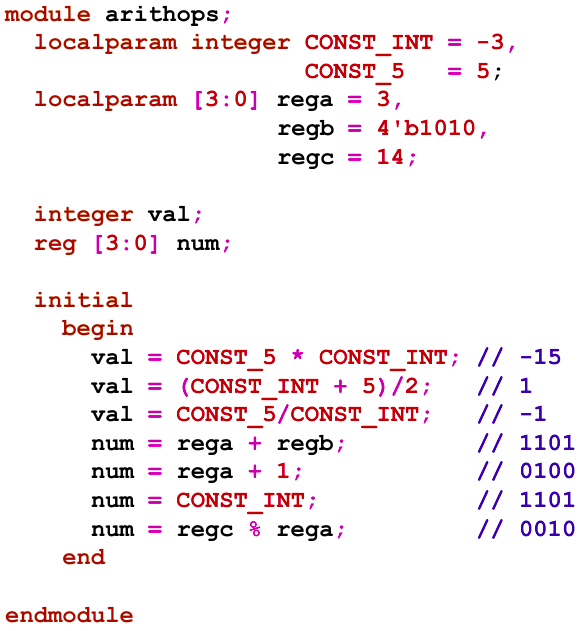
\includegraphics[width=0.45\textwidth]{img/05_arith.png}
\end{figure}
\end{multicols}
}
\end{frame}
\note{
\scriptsize{
The Verilog-1995 arithmetic operators are add, subtract, multiply, divide and modulus. Verilog-2001 added the power operator.
\newline

This example declares two \textit{integer} parameters, three 4-bit vector \textit{reg} parameters, an \textit{integer} variable and a 4-bit vector \textit{reg} variable, and performs some operations with them. See where integer division discards the fractional part. See where assigning 3 to an unsigned 4-bit vector \textit{reg} keeps the same rightmost four bits but now interprets the value as +13.
\newline

Some additional information about arithmetic operators:
\begin{itemize}
\item Any Z or X bit in either operand produces an unknown (X) result.
\item Integer division discards any remaining fractional part.
\item Division or modulo by 0 produces an unknown (X) result.
\item Raising 0 to a negative power produces an  result.
\item Raising a negative value to a real power produces an unspecified result. 
\end{itemize}

}
}

%%%%%%%%%%%%%%%%%%%%%%%%%%%%%%%%%%%%%%%%%%%%%%%%%%%%%%%%%%%%
\begin{frame}
\frametitle{Enhanced Signed Arithmetic}

\textbf{Verilog-2001}: New reserved word: \textbf{signed}
\begin{itemize}
\item \textcolor{purple}{signed} keyword treats literal, function, net, reg as signed
\item Arithmetic right shift operators maintains the sign of a value
\item \textcolor{purple}{\$signed} and \textcolor{purple}{\$unsigned} system functions cast value
\end{itemize}

\begin{figure}
    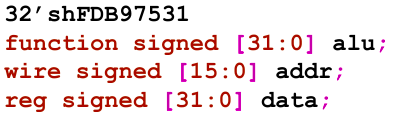
\includegraphics[width=0.45\textwidth]{img/05_enhanced.png}
\end{figure}
\end{frame}
\note{
\scriptsize{
The parser interprets an integer with no base specified as a signed value in 2's complement form: 

intA = -12/3;
\begin{itemize}
\item The left operand is a 32-bit signed value 12, negated
\item The expression result is -4
\end{itemize}
The parser interprets an integer with an unsigned base specifier as an unsigned value:

intA = -'\textbf{d}12/3;
\begin{itemize}
\item The left operand is a 32-bit unsigned value 12, negated.
\item The expression result is 1431655761
\end{itemize}
The parser interprets an integer with an signed base specifier as an signed value: 

intA = -4'\textbf{sd}12/3;
\begin{itemize}
\item The left operand is a 4-bit pattern of 12 (1100) interpreted as a signed number (-4) and then negated (4)
\item The expression result is 1
\end{itemize}

}
}

%%%%%%%%%%%%%%%%%%%%%%%%%%%%%%%%%%%%%%%%%%%%%%%%%%%%%%%%%%%%
\begin{frame}[fragile]
\frametitle{Signed Vectors}

\begin{multicols}{2}
\scriptsize{
\textcolor{purple}{signed} defines vector types as signed quantities.
\newline

2's complement:
\begin{itemize}
\item Also for function returns
\item Signed arithmetic for vectors is easier
\item Assignments between \verb+signed reg+ and \verb+integer+ types maintain sign information
\item Vector types can also be defined as \verb+unsigned+
\end{itemize}
By default, vectors are unsigned
\vfill
\columnbreak

\begin{figure}
    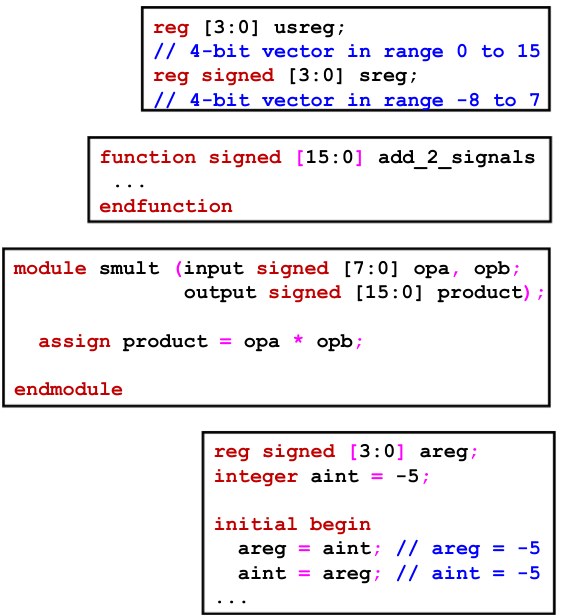
\includegraphics[width=0.45\textwidth]{img/05_signed.png}
\end{figure}
}
\end{multicols}
\end{frame}
\note{
For Verilog-2001, we can declare signed vectors. Vectors are by default unsigned. An unsigned vector is treated as signed for accesses through a signed port.

}
%%%%%%%%%%%%%%%%%%%%%%%%%%%%%%%%%%%%%%%%%%%%%%%%%%%%%%%%%%%%
\begin{frame}
\frametitle{Shift Operators}
\footnotesize{
Verilog-1995: \textcolor{purple}{logical shift \ \ \ \ $<<$\ \ \ $>>$}
\begin{itemize}
\item Ignores operand signs.
\item Fills extra bits with 0
\item Implements division or multiplication by powers of two
\end{itemize}

Verilog-2001: \textcolor{purple}{arithmetic shift \ \ \ \ $<<<$\ \ \ $>>>$}
\begin{itemize}
\item Ignores right operand sign
\item Left shift operates like logical left shift
\item Right shift preserves the left operand sign if the result is a signed expression.

\begin{figure}
    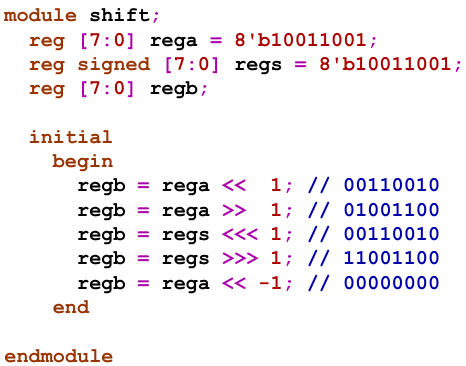
\includegraphics[width=0.45\textwidth]{img/05_shift.png}
\end{figure}
\end{itemize}
}
\end{frame}
\note{
\scriptsize{
The logical shift operators shift the left operand by the number of bit positions given by the right operand interpreted as a positive number, filling vacated bit positions with 0. We can use the logical shift operators to implement integer division or multiplication by powers of 2.
\newline

Verilog-2001 added the arithmetic shift operators. The arithmetic left shift operator operates exactly as does the logical left shift operator. The arithmetic right shift operator preserves the sign bit if the resulting expression is signed.
\newline

The example initializes an 8-bit vector \textbf{rega} to value 153(8'h99). Left-shifting this value once is equivalent to doubling its value, and placing the result back into a 8-bit vector \textit{reg}. The data truncates and the value gets back down to 50(8'h32). Right-shifting \textbf{rega} value once is equivalent to halving its value and losing the fractional part, so produces 76(8'h4c). Left-shifting by -1 is equivalent to left-shifting a veri large number of times, so produces 0. 

}
}

%%%%%%%%%%%%%%%%%%%%%%%%%%%%%%%%%%%%%%%%%%%%%%%%%%%%%%%%%%%%
\begin{frame}[fragile]
\frametitle{Relational Operators}
\scriptsize{
\begin{multicols}{2}
\begin{Verbatim}[commandchars=\\\{\}, tabsize=2]
\textcolor{purple}{less than                 <}
\textcolor{purple}{greater than              >}
\textcolor{purple}{less than or equal to     <=}
\textcolor{purple}{greater than or equal to  >=}
\end{Verbatim}

The result is:
\begin{itemize}
\item \verb+1'b0+ if the relation is false
\item \verb+1'b1+ if the relation is true
\item \verb+1'bX+ if either operand contains any Z or X bits
\end{itemize}

\vfill
\columnbreak

\begin{figure}
    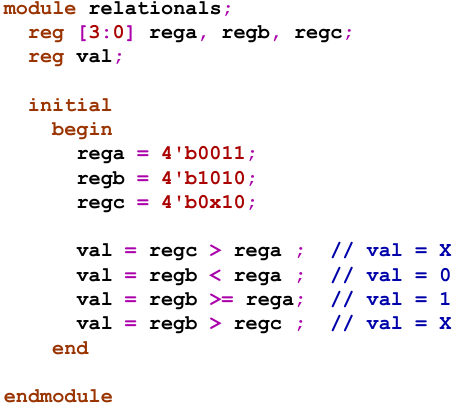
\includegraphics[width=0.45\textwidth]{img/05_relation.png}
\end{figure}
\end{multicols}
}
\end{frame}
\note{
\scriptsize{
If at least one operand is unsigned, the comparison treats both operands as unsigned and zero-extends a smaller operand to match the width of a wider operand.
\newline

If both operands are signed integer quantities, the operation sign-extends a smaller operand to match the width of a wider operand and treats the comparison as a signed integer comparison.
\newline

If at least one operand is real, the operation if necessary converts the other operand to real and treats the comparison as a real comparison.
\newline

The result is 0 if the relation is false and 1 if the relation is true. Any high-impedance(z) or unknown(x) bit in either operand produces an unknown result regardless of the truth of the relation. 

}
}
%%%%%%%%%%%%%%%%%%%%%%%%%%%%%%%%%%%%%%%%%%%%%%%%%%%%%%%%%%%%
\begin{frame}[fragile]
\frametitle{Logical Equality and Case Equality Operators}
\scriptsize{
\begin{multicols}{2}

\begin{Verbatim}[commandchars=\\\{\}, tabsize=2]
\textcolor{purple}{logical equality ==}
\end{Verbatim}

\begin{itemize}
\item Result can be unknown
\end{itemize}

\begin{figure}
    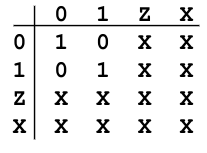
\includegraphics[width=0.2\textwidth]{img/05_equal0.png}
\end{figure}
\begin{Verbatim}[commandchars=\\\{\}, tabsize=2]
\textcolor{purple}{case equality ==}
\end{Verbatim}
\begin{itemize}
\item Result is always known
\end{itemize}
\begin{figure}
    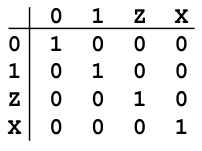
\includegraphics[width=0.2\textwidth]{img/05_equal1.png}
\end{figure}
\vfill
\columnbreak

\begin{figure}
    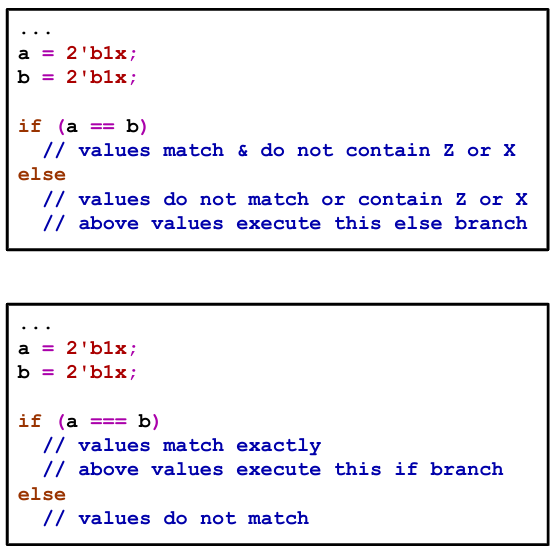
\includegraphics[width=0.45\textwidth]{img/05_equal2.png}
\end{figure}
\end{multicols}
}
\end{frame}
\note{
\scriptsize{
The difference between logical and case equality is the handling of high-impedance and unknown values. The logical equality treats high-impedance and unknown bits as truly unknown bit values, while the case equality treats high-impedance and unknown bits as values to be matched. A case equality operation thus always produces a 0 or a 1 result and never an unknown result.
\newline

The case equality operator gets its name from the fact that the \textit{case} statement, which we will see later, matches items in the same manner. Some people call it the "identity" operator because it checks that the bits are identical instead of that their values are the same.

}
}

%%%%%%%%%%%%%%%%%%%%%%%%%%%%%%%%%%%%%%%%%%%%%%%%%%%%%%%%%%%%
\begin{frame}[fragile]
\frametitle{More about Equality Operators}
\scriptsize{
\begin{multicols}{2}

\begin{Verbatim}[commandchars=\\\{\}, tabsize=2]
\textcolor{purple}{logical equality   ==}
\textcolor{purple}{logical inequality !=}
\textcolor{purple}{case equality      ===}
\textcolor{purple}{case inequality    !==}
\end{Verbatim}
\begin{itemize}
\item For logical equalities result can be unknown
\end{itemize}

\begin{figure}
    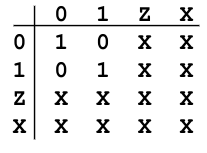
\includegraphics[width=0.2\textwidth]{img/05_equal0.png}
\end{figure}

\begin{itemize}
\item For case equalities result is always known
\end{itemize}
\begin{figure}
    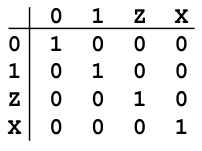
\includegraphics[width=0.2\textwidth]{img/05_equal1.png}
\end{figure}
\vfill
\columnbreak
\begin{figure}
    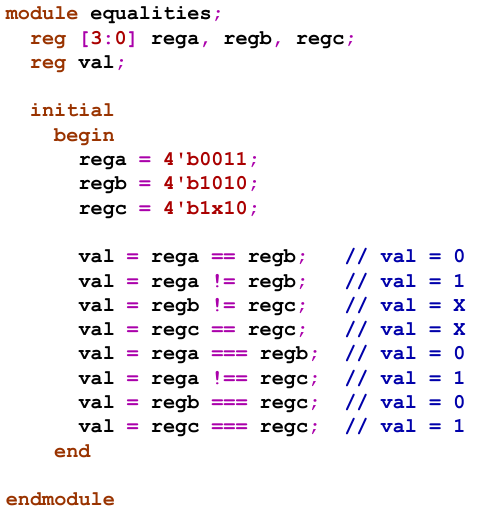
\includegraphics[width=0.45\textwidth]{img/05_inequality.png}
\end{figure}

\end{multicols}
}
\end{frame}
\note{
\scriptsize{
Here is another example illustrating the difference between logical and case equality operators.
\newline

The difference between logical and case equality is the handling of high-impedance and unknown values. The logical equality treats high-impedance and unknown bits as truly unknown bit values, while the case equality treats high-impedance and unknown bits as values to be matched. A case equality operation thus always produces a 0 or a 1 result and never an unknown result.

}
}

%%%%%%%%%%%%%%%%%%%%%%%%%%%%%%%%%%%%%%%%%%%%%%%%%%%%%%%%%%%%
\begin{frame}[fragile]
\frametitle{Conditional Operator}
\begin{multicols}{2}
\begin{Verbatim}[commandchars=\\\{\}, tabsize=2]
\textcolor{purple}{conditional ?:}
\end{Verbatim}
\begin{figure}
    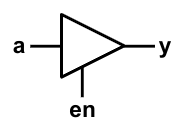
\includegraphics[width=0.2\textwidth]{img/05_cond0.png}
\end{figure}
\vfill
\columnbreak

\begin{figure}
    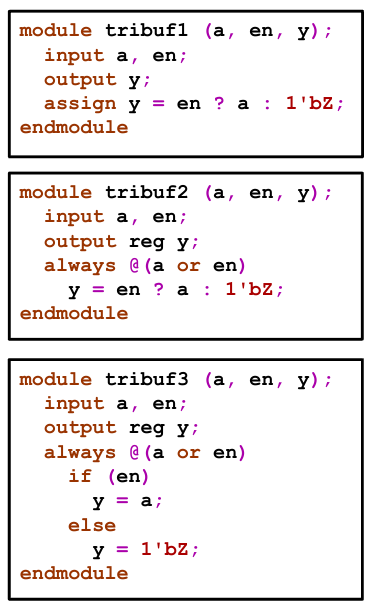
\includegraphics[width=0.45\textwidth]{img/05_cond1.png}
\end{figure}
\end{multicols}
\end{frame}
\note{
\scriptsize{
The conditional operator is a ternary operator. It has three operands.
\begin{itemize}
\item If the first operand, the condition expression, is 1, then the operation result is the value of the second operand.
\item If the first operand is 0, then the operation result is the value of the third operand.
\item If the first operand is unknown (X), then the operation result is the value of the second operand merged with the value of the third operand so that if any bit position has the same value in both operands, then that bit position of the result also has that value.
\end{itemize}
So the conditional operator selects between two operands like a 2-to-1  multiplexor.
\newline

The operands can be any expression. It is very common to nest conditional operations.

}
}

%%%%%%%%%%%%%%%%%%%%%%%%%%%%%%%%%%%%%%%%%%%%%%%%%%%%%%%%%%%%
\begin{frame}[fragile]
\frametitle{Concatenation Operator}
\scriptsize{
\begin{multicols}{2}
\begin{Verbatim}[commandchars=\\\{\}, tabsize=2]
\textcolor{purple}{concatenation \{\}}
\end{Verbatim}
Can select and join bits from different vectors to form a new vector:
\begin{itemize}
\item Forms unsigned expression
\end{itemize}
Can reorganize vector bits to form a new vector:
\begin{itemize}
\item Endian swaps / reverse / rotate
\end{itemize}
Can use on either side of an assignment!
\vfill
\columnbreak

\begin{figure}
    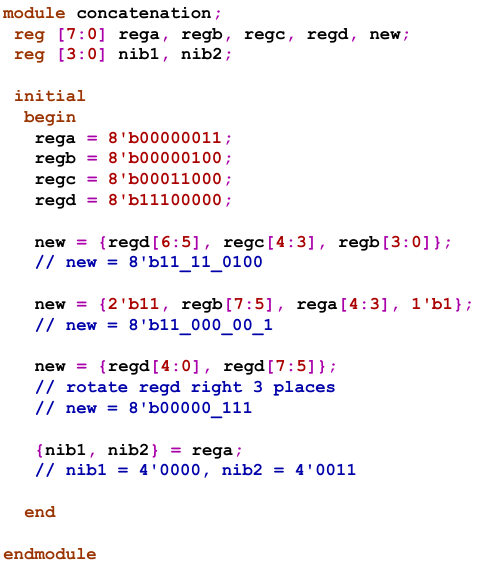
\includegraphics[width=0.45\textwidth]{img/05_concat.png}
\end{figure}
\end{multicols}
}
\end{frame}
\note{
A concatenation operation joins together the bits of one or more comma-separated operands. We must size literal constant operands so that the operation can determine exactly where to place each bit.
\newline

Literals in a concatenation must be explicitly sized so that all the bits go into the correct position.
\newline

Here are some examples that fail to size their operands:

a[7:0] = \{5'b01010, 2\}; // decimal value 2 is unsized

c[3:0] = \{3'b011, 'b0\}; // binary value 'b0 is unsized 
}

%%%%%%%%%%%%%%%%%%%%%%%%%%%%%%%%%%%%%%%%%%%%%%%%%%%%%%%%%%%%
\begin{frame}[fragile]
\frametitle{Replication Operator}
\scriptsize{
\begin{multicols}{2}
\begin{Verbatim}[commandchars=\\\{\}, tabsize=2]
\textcolor{purple}{replication \{\{\}\}}
\end{Verbatim}

\begin{itemize}
\item Reproduces a concatenation a set number of times
\end{itemize}


Syntax: 
\begin{Verbatim}[commandchars=\\\{\}, tabsize=2]
\{\textit{const_expr} \{\textit{sized_expr}\}\}
\end{Verbatim}

\begin{itemize}
\item The constant number of repetitions must not have \verb+z+ or \verb+x+ values.
\end{itemize}
\vfill
\columnbreak

\begin{figure}
    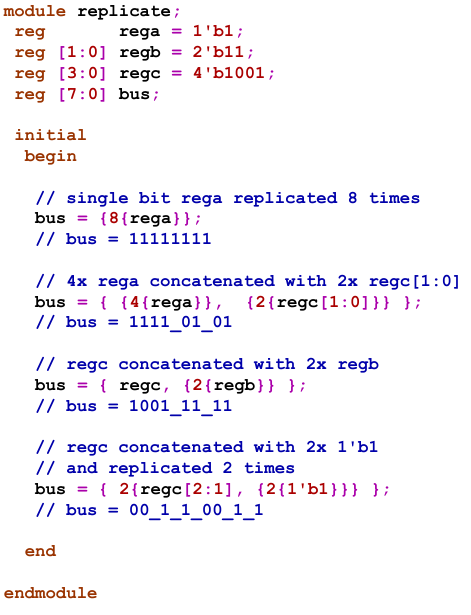
\includegraphics[width=0.45\textwidth]{img/05_replica.png}
\end{figure}

\end{multicols}
}
\end{frame}
\note{
\scriptsize{
A replication operation replicates a concatenation a  number of times. A replication operation applies only to a concatenation. We will not see it in any other context. The replication count cannot have any high-impedance (z) or unknown (x) values.
\newline

This example:
\begin{itemize}
\item 1st: Replicates the value of the single-bit \textbf{rega} variable value eight times to form a 8-bit value it assigns to the bus variable;
\item 2nd: Concatenates four replications of the value of the single-bit \textbf{rega} variable with two replications of the value of the lowest two bits of the \textbf{regc} variable to form an 8-bit value it assigns to the bus variable;
\item 3rd: Concatenates the value of the four-bit \textbf{regc} variable with two replications of the value of the two-bit \textbf{regb} variable to form an 8-bit value it assigns to the bus variable;
\item 4th: Concatenates the value of the middle two bits of the \textbf{regc} variable with two replications of the sized literal constant 1'b1, and replicates that 4-bit concatenation twice to form an 8-bit value it  to the bus variable. 
\end{itemize} 

}
}

%%%%%%%%%%%%%%%%%%%%%%%%%%%%%%%%%%%%%%%%%%%%%%%%%%%%%%%%%%%%
\begin{frame}
\frametitle{Reference: Operator Precedence High to Low}
\begin{figure}
    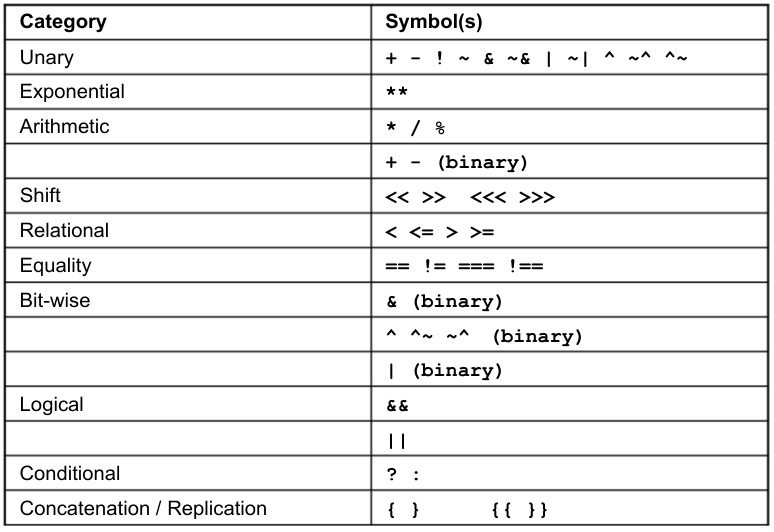
\includegraphics[width=0.75\textwidth]{img/05_precedence.png}
\end{figure}
\textbf{Reliance on operator precedence may make our code unreadable - use parentheses!}
\end{frame}
\note{
\scriptsize{
Out reliance on operator precedence can make our code unreadable to the great majority of people that do not memorize this table. Our co-workers will appreciate out appropriate use of parenthesized expressions.
\newline

Group the following expression:

a ? \~{} b $*$ c \textless\textless\ d : e \textless\ f \^{} g \textbar\textbar\ h

Solution:

a ? ((\~{} b $*$ c) \textless\textless\ d) : (((e \textless\ f) \^{} g) \textbar\textbar\ h)
}
}

%%%%%%%%%%%%%%%%%%%%%%%%%%%%%%%%%%%%%%%%%%%%%%%%%%%%%%%%%%%%
\begin{frame}
\frametitle{Module Summary}
\scriptsize{
Now we can appropriately and correctly use Verilog operators. This module presented the following Verilog operators:
\begin{itemize}
\item Reduction unary operators that perform a bit-wise operation across all bits of a single operand
\item Arithmetic binary operators that preserve signage
\item Shift binary operators - the right shift optionally preserves signage
\item Relational binary operators
\item Logical and case equality binary operators
\item Bit-wise binary operators that perform individual logical operations on each bit position of two vectors
\item Logical unary operator and binary operators that treat their operand as logical values
\item Conditional ternary operator that selects between two operands based on the logical value of the third operand
\item Concatenation operator that concatenates scalar or vector operands to create a new vector
\item Replication operator that replicates a concatenation a fixed number of times
\end{itemize}

}
\end{frame}

%%%%%%%%%%%%%%%%%%%%%%%%%%%%%%%%%%%%%%%%%%%%%%%%%%%%%%%%%%%%
\begin{frame}
\frametitle{Module Review}
\begin{enumerate}
\item How wide is the result of a logical \&\& operation?
\item Explain the difference between \&\& and \& operators.
\item TRUE or FALSE: We must explicitly size literals in concatenation
\item Given the statement \textbf{regx = 4'b0101;} what is the value of:
 
\textbf{bus = \{2 \{regx[3:1], \{3\{1'b0, regx[0]\}\}\} \}}
\end{enumerate}
\end{frame}
\note{
\scriptsize{
\begin{enumerate}
\item How wide is the result of a logical \&\& operation?

\begin{itemize}
\item \scriptsize{The logical \&\& operator reduces each operand to a single-bit (1'b1, 1'b0 or 1'bx), then ANDs these bits together to give a single-bit result.}
\end{itemize}

\item Explain the difference between \&\& and \& operators.
\begin{itemize}
\item \scriptsize{The logical \&\& operator reduces each operand to a single-bit (1'b1, 1'b0 or 1'bx), then ANDs these bits together to give a single-bit result.
The bitwise \& operator does bit-by-bit AND of its operands, from LSB to MSB, producing a result which is the same width as the longest operand.}
\end{itemize}

\item TRUE or FALSE: We must explicitly size literals in concatenation

\begin{itemize}
\item \scriptsize{TRUE. All operands in a concatenation must have a size. }
\end{itemize}

\item Given the statement \textbf{regx = 4'b0101;} what is the value of:
 
\textbf{bus = \{2 \{regx[3:1], \{3\{1'b0, regx[0]\}\}\} \}}

\begin{itemize}
\item \scriptsize{bus = 18'b010\_01\_01\_01\_010\_01\_01\_01; }
\end{itemize}
\end{enumerate}
}
}

%%%%%%%%%%%%%%%%%%%%%%%%%%%%%%%%%%%%%%%%%%%%%%%%%%%%%%%%%%%%
\begin{frame}
\frametitle{Module Exercise}
Fix this code so that it preserves the sign of the value.
\begin{figure}
    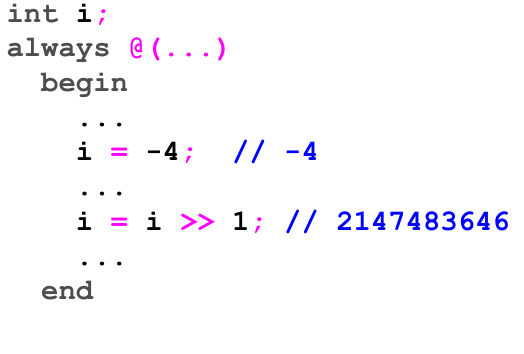
\includegraphics[width=0.45\textwidth]{img/05_exe.png}
\end{figure}
\end{frame}
\note{
Solution:
\begin{figure}
    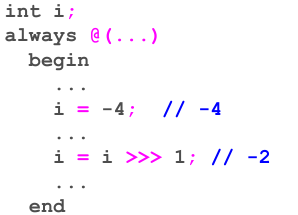
\includegraphics[width=0.45\textwidth]{img/05_exe_sol.png}
\end{figure}
}

%%%%%%%%%%%%%%%%%%%%%%%%%%%%%%%%%%%%%%%%%%%%%%%%%%%%%%%%%%%%
\begin{frame}
\frametitle{Lab}
Lab 6-1: Modeling the arithmetic logic Unit
\begin{itemize}
\item use Verilog operators while describing a parametrized-width arithmetic logic unit (ALU)

\begin{figure}
    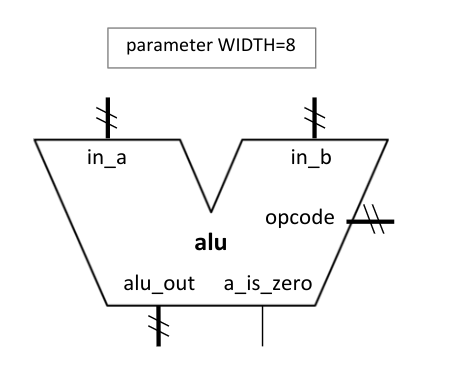
\includegraphics[width=0.45\textwidth]{img/05_lab.png}
\end{figure}


\end{itemize}
\end{frame}

%%%%%%%%%%%%%%%%%%%%%%%%%%%%%%%%%%%%%%%%%%%%%%%%%%%%%%%%%%%%
\begin{frame}
\frametitle{Test Your Understanding - 1}
A new team member coded the expression (-1 \textgreater\textgreater\textgreater\ -1) . We have to explain to our team what the result would be. What would it be?
\begin{itemize}
\item[$\square$] 0
\item[$\square$] -2
\item[$\square$] 2147583647
\item[$\square$] -1
\item[$\square$] 4294967294
\end{itemize}
\end{frame}
\note{
A new team member coded the expression (-1 \textgreater\textgreater\textgreater\ -1) . We have to explain to our team what the result would be. What would it be?
\begin{itemize}
\item[$\square$] 0
\item[$\square$] -2
\item[$\square$] 2147583647
\item[$\boxtimes$] -1
\item[$\square$] 4294967294
\end{itemize}
}

%%%%%%%%%%%%%%%%%%%%%%%%%%%%%%%%%%%%%%%%%%%%%%%%%%%%%%%%%%%%
\begin{frame}
\frametitle{Test Your Understanding - 2}
We code a replication expression. The replication value must be a constant expression.
\begin{itemize}
\item[$\square$] True
\item[$\square$] False
\end{itemize}
\end{frame}
\note{
We code a replication expression. The replication value must be a constant expression.
\begin{itemize}
\item[$\boxtimes$] True
\item[$\square$] False
\end{itemize}
}

%%%%%%%%%%%%%%%%%%%%%%%%%%%%%%%%%%%%%%%%%%%%%%%%%%%%%%%%%%%%
\begin{frame}
\frametitle{Test Your Understanding - 3}
We are verifying the DUT response to our stimulus. Which one or more operator classes can you NOT use because they can produce an unknown result if an operand is unknown>
\begin{itemize}
\item[$\square$] arithmetic ($+$ $-$ $*$ $/$)
\item[$\square$] case equality ($===$ $!==$)
\item[$\square$] logical equality ($==$ $!=$)
\item[$\square$] reduction (\&\ \textbar\ \^{})
\item[$\square$] conditional (?:)
\item[$\square$] relational (\textless\ \textless= \textgreater= \textgreater)
\end{itemize}
\end{frame}
\note{
We are verifying the DUT response to our stimulus. Which one or more operator classes can you NOT use because they can produce an unknown result if an operand is unknown>
\begin{itemize}
\item[$\boxtimes$] arithmetic ($+$ $-$ $*$ $/$)
\item[$\square$] case equality ($===$ $!==$)
\item[$\boxtimes$] logical equality ($==$ $!=$)
\item[$\boxtimes$] reduction (\&\ \textbar\ \^{})
\item[$\boxtimes$] conditional (?:)
\item[$\boxtimes$] relational (\textless\ \textless= \textgreater= \textgreater)
\end{itemize}
}

%%%%%%%%%%%%%%%%%%%%%%%%%%%%%%%%%%%%%%%%%%%%%%%%%%%%%%%%%%%%
\begin{frame}
\frametitle{Test Your Understanding - 4}
We are coding a signal-processing algorithm. Which one or more classes of operators can we use because they can produce signed results.
\begin{itemize}
\item[$\square$] concatenation
\item[$\square$] bitwise
\item[$\square$] shift
\item[$\square$] arithmetic
\end{itemize}
\end{frame}
\note{
We are coding a signal-processing algorithm. Which one or more classes of operators can we use because they can produce signed results.
\begin{itemize}
\item[$\square$] concatenation
\item[$\boxtimes$] bitwise
\item[$\boxtimes$] shift
\item[$\boxtimes$] arithmetic
\end{itemize}
}

%%%%%%%%%%%%%%%%%%%%%%%%%%%%%%%%%%%%%%%%%%%%%%%%%%%%%%%%%%%%
\begin{frame}
\frametitle{Test Your Understanding - 5}
Conditional operators is the only "\_\_\_\_\_\_\_" operator in most programing languages.
\begin{itemize}
\item[$\square$] ternary
\item[$\square$] unary
\item[$\square$] quaternary
\item[$\square$] binary
\end{itemize}
\end{frame}
\note{
Conditional operators is the only "\_\_\_\_\_\_\_" operator in most programing languages.
\begin{itemize}
\item[$\boxtimes$] ternary
\item[$\square$] unary
\item[$\square$] quaternary
\item[$\square$] binary
\end{itemize}
}

%%%%%%%%%%%%%%%%%%%%%%%%%%%%%%%%%%%%%%%%%%%%%%%%%%%%%%%%%%%%
\begin{frame}
\frametitle{Test Your Understanding - 6}
Select the following expression(s) that are illegal in Verilog.
\begin{itemize}
\item[$\square$] A \&\&\ B
\item[$\square$] A \textbar\textbar\ B
\item[$\square$] A \&\ \&\ B
\item[$\square$] A \&\ (\&B)
\item[$\square$] A \textbar\ \textbar\ B
\item[$\square$] A \textbar\ (\textbar B)
\end{itemize}
\end{frame}
\note{
Select the following expression(s) that are illegal in Verilog.
\begin{itemize}
\item[$\square$] A \&\&\ B
\item[$\square$] A \textbar\textbar\ B
\item[$\boxtimes$] A \&\ \&\ B
\item[$\square$] A \&\ (\&B)
\item[$\boxtimes$] A \textbar\ \textbar\ B
\item[$\square$] A \textbar\ (\textbar B)
\end{itemize}
}

\end{document}
